\begin{align*}
    \polynomialP{2}{X}{0} &= 0 \\
    \polynomialP{2}{X}{1} &= 30X^2 - 60X + 31 \\
    \polynomialP{2}{X}{2} &= 150X^2 - 540X + 512 \\
    \polynomialP{2}{X}{3} &= 420X^2 - 2160X + 2943 \\
    \polynomialP{2}{X}{4} &= 900X^2 - 6000X + 10624 \\
    \polynomialP{2}{X}{5} &= 1650X^2 - 13500X + 29375 \\
    \polynomialP{2}{X}{6} &= 2730X^2 - 26460X + 68256 \\
    \polynomialP{2}{X}{7} &= 4200X^2 - 47040X + 140287 \\
    \polynomialP{2}{X}{8} &= 6120X^2 - 77760X + 263168 \\
    \polynomialP{2}{X}{9} &= 8550X^2 - 121500X + 459999 \\
    \polynomialP{2}{X}{10} &= 11550X^2 - 181500X + 760000 \\
    \polynomialP{2}{X}{11} &= 15180X^2 - 261360X + 1199231 \\
    \polynomialP{2}{X}{12} &= 19500X^2 - 365040X + 1821312 \\
    \polynomialP{2}{X}{13} &= 24570X^2 - 496860X + 2678143 \\
    \polynomialP{2}{X}{14} &= 30450X^2 - 661500X + 3830624 \\
    \polynomialP{2}{X}{15} &= 37200X^2 - 864000X + 5349375 \\
    \polynomialP{2}{X}{16} &= 44880X^2 - 1109760X + 7315456 \\
    \polynomialP{2}{X}{17} &= 53550X^2 - 1404540X + 9821087 \\
    \polynomialP{2}{X}{18} &= 63270X^2 - 1754460X + 12970368 \\
    \polynomialP{2}{X}{19} &= 74100X^2 - 2166000X + 16879999 \\
    \polynomialP{2}{X}{20} &= 86100X^2 - 2646000X + 21680000
\end{align*}
\begin{figure}[H]
    \centering
    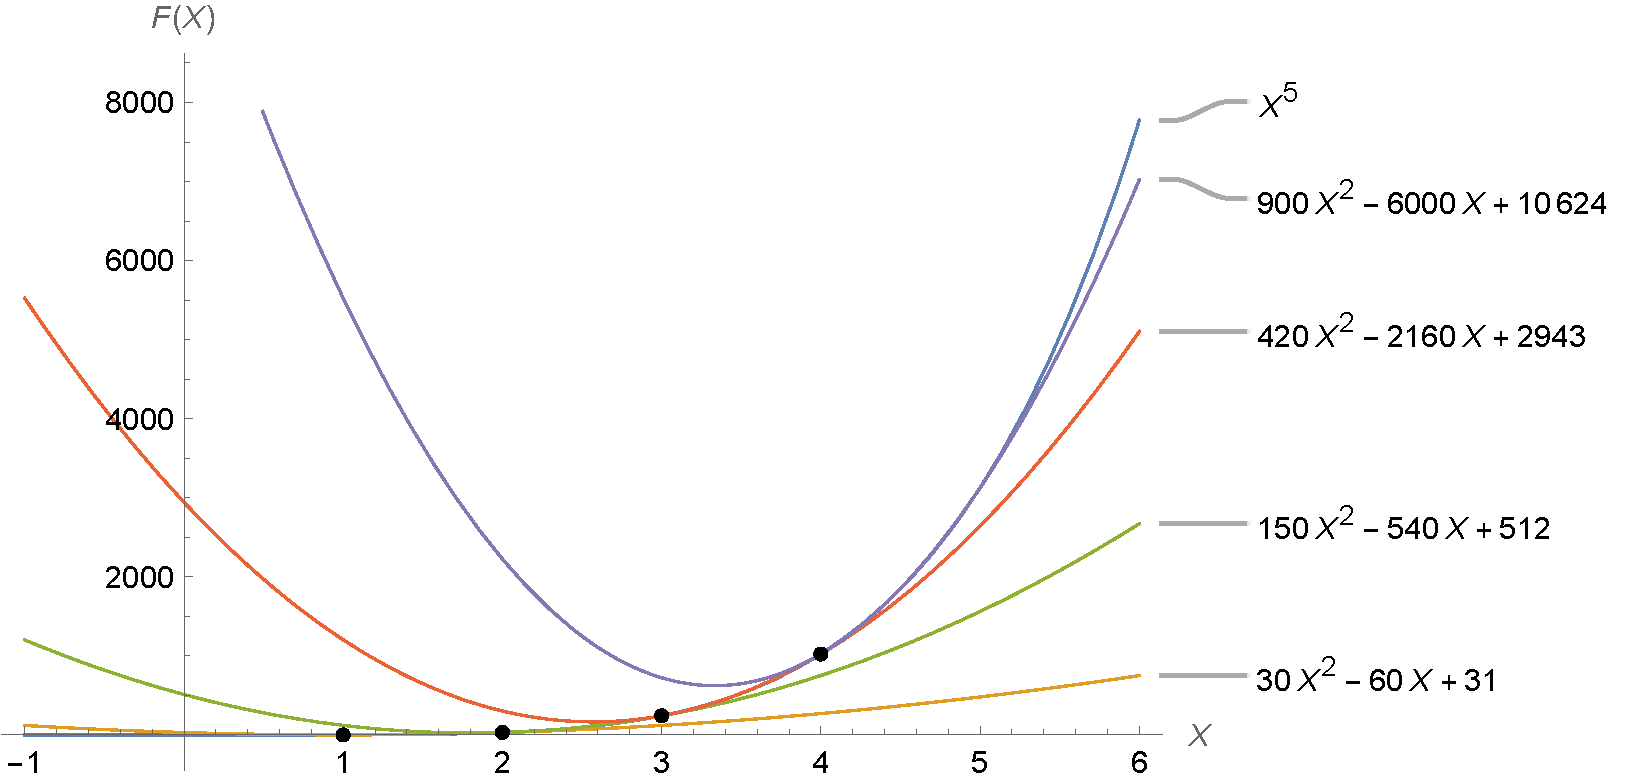
\includegraphics[width=1\textwidth]{sections/images/03_fifth_power_with_p_1_n_k}
    ~\caption{Polynomials P(2, n, k)}\label{fig:figure3}
\end{figure}
